%!TEX root = ../my_thesis.tex
\chapter{Processeurs personnalisés à faible consommation pour le décodage SC} % (fold)
\label{chap:tensilica}

\vspace*{\fill}
\minitocTITI
\vspace*{\fill}
\newpage

\section*{Introduction}
Les implémentations logicielles des fonctions de traitement du signal dans les infrastructures de communication radio sont encouragées pour tendre vers un réseau virtualisé de type Cloud-RAN. De telles implémentations sont présentées pour les algorithmes de décodage polaire à liste dans le chapitre précédent. De hauts débits peuvent être atteints, et la flexibilité et la généricité de ces décodeurs est très importante. En utilisant des processeurs visant des systèmes électroniques embarqués, ces implémentations peuvent également gagner en efficacité énergétique.

Toutefois, les processeurs à usage général incluent de nombreuses unités matérielles destinées à réaliser efficacement de nombreuses et diverses applications. Mais ces unités matérielles ne sont pas utilisées dans certaines de ces applications. Par exemple, dans les algorithmes de décodage de canal, toutes les unités de calcul à point flottant sont inutiles puisqu'une représentation des données interne par virgule fixe est suffisante. Ces unités matérielles consomment de l'énergie inutilement. Le profilage d'un décodeur polaire montre que la majeure partie du temps d'exécution est passé à réaliser un ensemble restreint de fonctions élémentaires. De plus, une part significative des instructions exécutées correspond à des opérations de sauvegarde et de chargement de données dans les registres.

Ces observations poussent à envisager la conception d'un processeur programmable qui exclurait les unités matérielles inutiles des processeurs à usage général, tout en intégrant des unités de calculs spécialisées dans la réalisation efficace des fonctions élémentaires de décodage de codes polaires. Ce type de processeurs entre dans la catégorie des processeurs à jeu d'instructions spécifique à l'application (ASIP: Application Specific Instruction-set Processor).

Les Chapitres \ref{chap:tensilica} et \ref{chap:tta} de ce manuscrit présentent deux architectures de processeurs ASIP spécialisées dans le décodage de code polaire. Ces deux architectures ont été conçues selon des méthodologies de conception différentes. Dans la Section \ref{sec:asips}, le concept d'ASIP est introduit, et la méthodologie utilisée pour la première architecture est décrite. Dans la Section \ref{tensilica_design}, la conception de l'ASIP est détaillée. Enfin les résultats d'implémentation et les performances de l'architecture en termes de débit, latence, complexité et consommation énergétiques sont présentés et discutés dans la Section \ref{sec:tensilica_res}.


\section{Les processeurs à jeu d'instructions spécifiques à l'application}
\label{sec:asips}

L'architecture ASIP que nous avons développée est basée sur une processur de type RISC (Reduced Instruction Set Computer). Dans une première sous-section, les principes des architectures RISC sont présentés. Le concept d'ASIP sera ensuite introduit ainsi que leurs deux grandes méthodologies de conception. Le flot de conception de l'outil logiciel utilisé pour concevoir notre ASIP sera ensuite présenté.

\subsection{Les processeurs RISC}

\begin{figure}[t]
\centering
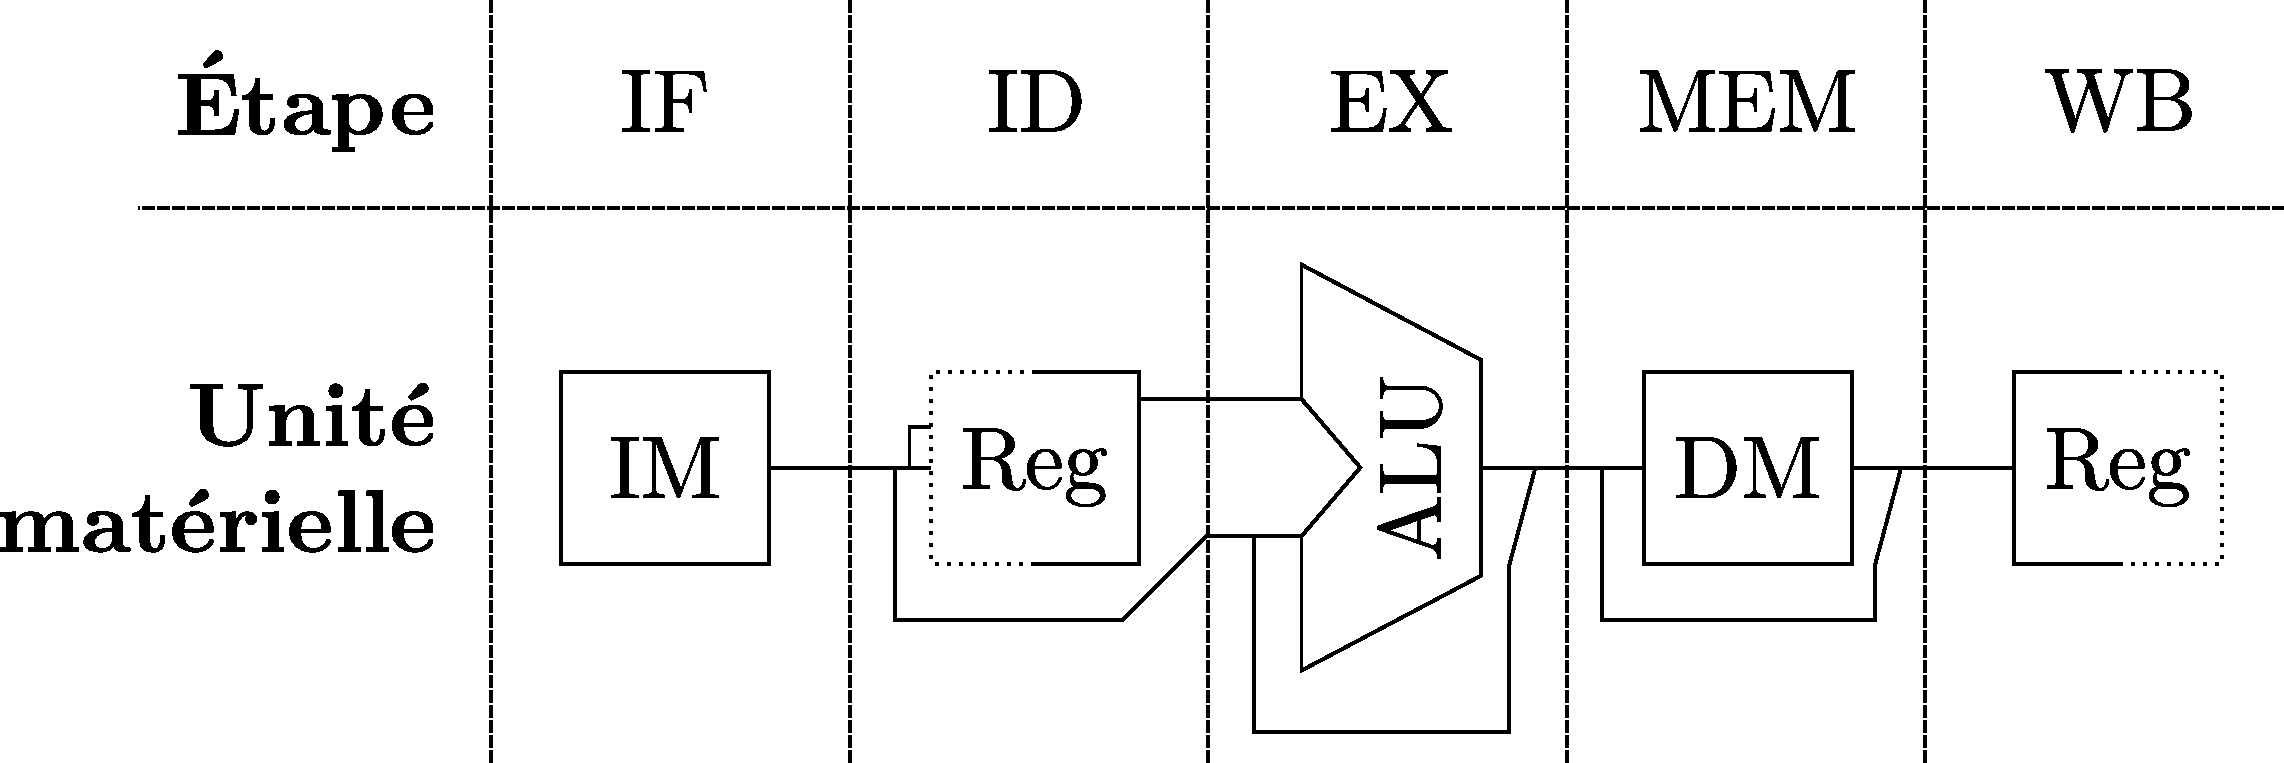
\includegraphics[width=\textwidth]{main/ch3_fig/stages}
\caption{\'Etages d'un processeur RISC}
\end{figure}

Dans le domaine de l'embarqué, les processeurs utilisés sont souvent de type RISC. Cette classe de processeurs a été introduite dans \cite{hennessy2011computer}. Par une analyse statistique et quantitative des applications traitées par les architectures de processeurs, les auteurs ont abouti à une microarchitecture de processeurs composée de 5 étages. Une unité matérielle est associée à chacun des étages, comme montré dans la figure \ref{fig:stages}.

\begin{itemize}
  \item Le premier étage est l'étage de \textbf{chargement de l'instruction} (IF : Instruction Fetch) depuis la \textit{mémoire d'instruction} (IM : Instruction Memory). A chaque coup d'horloge, une nouvelle instruction est chargée dans un registre spécialisé, nommé registre d'instruction. L'adresse en mémoire de l'instruction à lire est déterminée par le pointeur d'instruction, registre incrémenté automatiquement à chaque coup d'horloge. L'instruction contient l'opération qui sera effectuée par le processeur dans les étages suivants. Il peut s'agir d'instructions arithmétiques et logiques, d'instructions de chargement et de sauvegarde depuis et vers la mémoire, ou bien d'instructions de branchement et de sauts, afin de se déplacer dans la mémoire d'instructions. Elle contient également des informations sur les registres qui doivent être lus ou écrits, ainsi que des adresses mémoire dans le cas d'opérations de chargement ou de sauvegarde.

  \item Le deuxième étage est le \textbf{décodage de l'instruction} (ID : Instruction Decode) et de lecture du \textit{fichier de registre} (RF : Register File) spécifié(s) par l'instruction. Divers signaux de contrôle, qui seront utilisés dans les étages suivants, sont générés, selon l'instruction décodée.

  \item Le troisième étage est l'étage d'\textbf{exécution} (EX : Execution) dans lequel l'unité arithmétique et logique (ALU : Arithmetical and Logical Unit) effectue des opérations arithmétiques (+,-,*,/) et logiques (AND, OR, XOR,...). Ces opérations peuvent servir a effectué des calculs d'adresse relative ou a réaliser des opérations sur deux entrées. Ces deux entrées peuvent être deux registres ou bien un registre et une valeur immédiate intégrée dans l'instruction elle-même.

  \item Le quatrième étage est l'étage d'\textbf{accès à la mémoire}. S'il s'agit d'un chargement, une donnée est lue dans la \textit{mémoire de donnée} (DM : Data Memory) à l'adresse spécifiée par un des registres. S'il s'agit d'une sauvegarde, la valeur d'un deuxième registre est écrite dans la DM.

  \item Le cinquième est l'étape d'\textbf{écriture différée} (WB : write-back). Cette étage permet d'écrire le résultat dans le fichier de registre, que ce soit le résultat d'une opération effectuée par l'ALU ou bien une donnée lue dans la DM.
\end{itemize}

\begin{figure}[t]
\centering
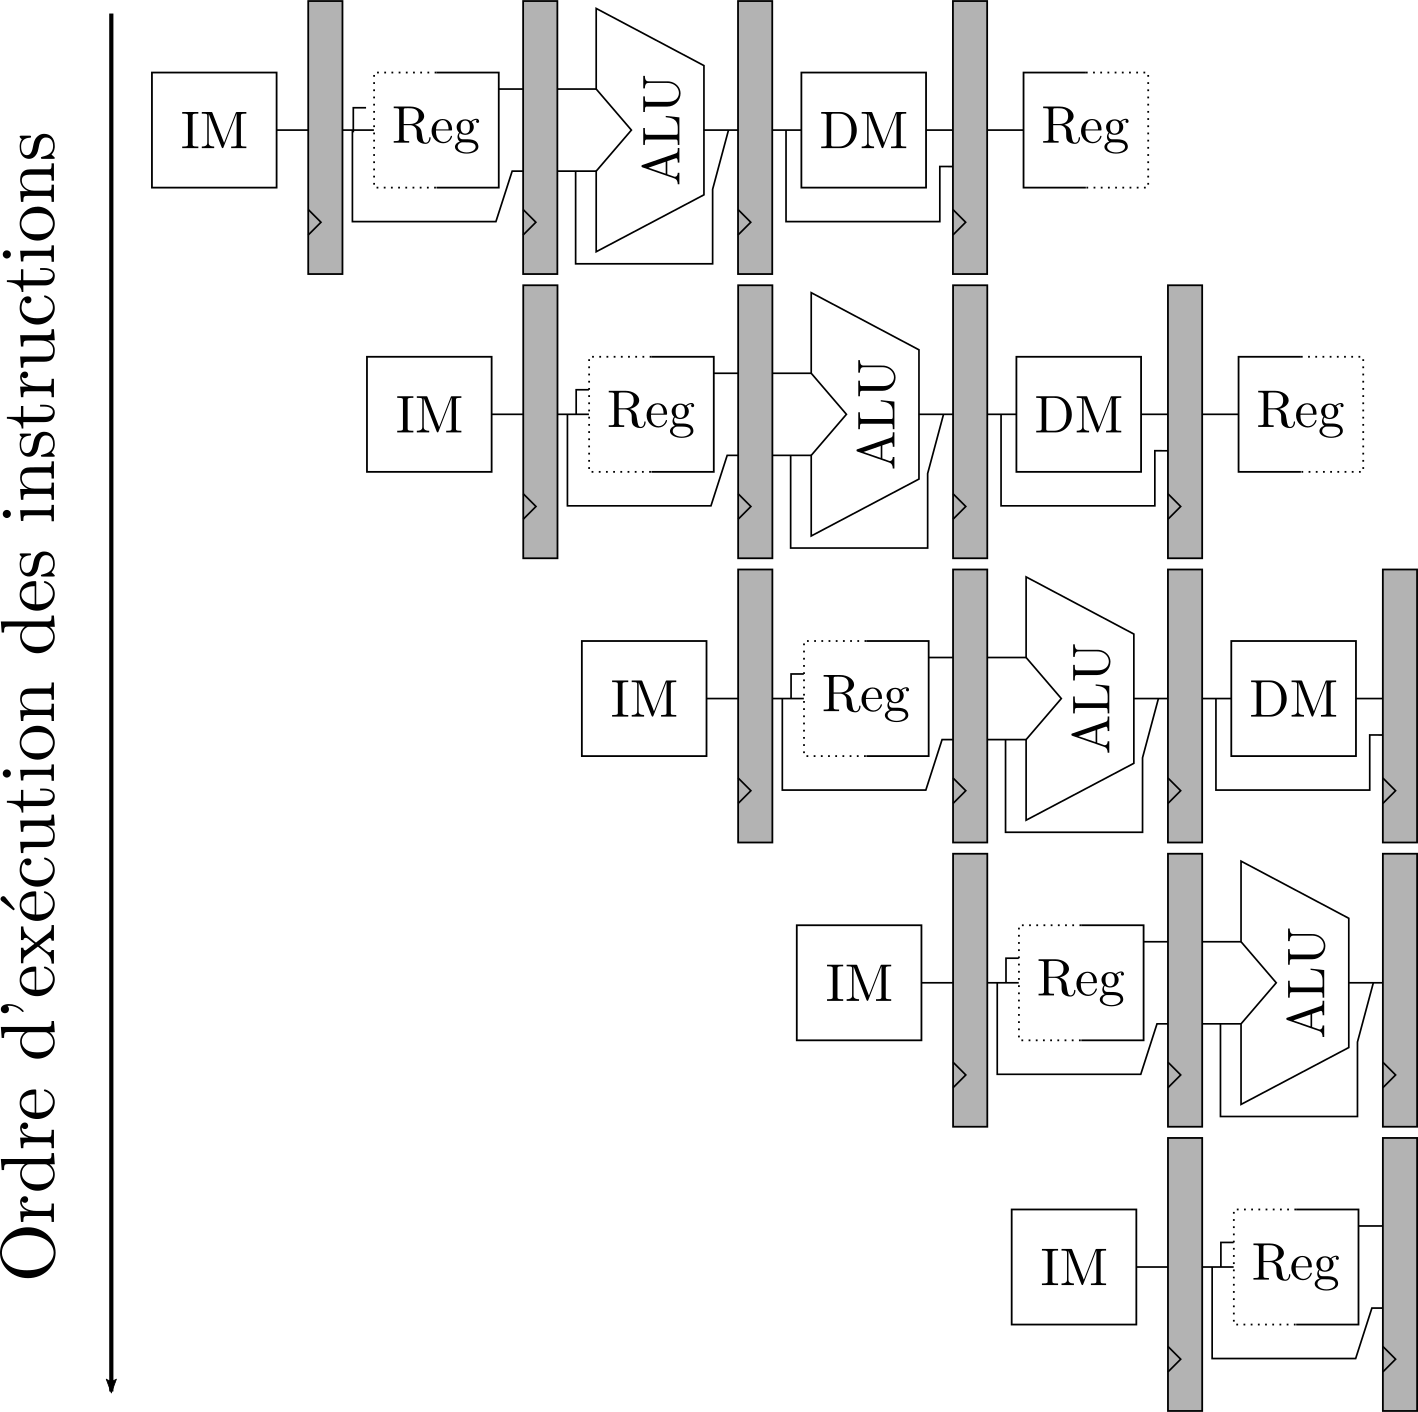
\includegraphics[width=0.75\textwidth]{main/ch3_fig/pipelines}
\caption{Pipeline à 5 étages}
\end{figure}


L'ajout de registres de pipeline représentés dans la Figure~\ref{fig:pipelines} permet d'isoler chacun des étages. AInsi à chaque cycle d'horloge, représenté ici par les lignes horizontales, une instruction est transmise d'un étage au suivant. Si une instruction est initiée à chaque coup d'horloge, alors la performance du processeur sera 5 fois supérieure à celle d'un processeur sans pipeline.






\subsection{Les processeurs à jeu d'instructions spécifiques à l'application}



Le jeu d'instructions (ISA : )
- Configurabilité et extensivité


\subsection{Le flot de conception Tensilica}
\label{tensilica_design}
\section{Un ASIP dédié au décodage de codes polaires}
\subsection{Implémentations matérielles de l'algorithme SC}
\label{subsec:sota_sc}
\subsection{Configuration}
\subsubsection{Architecture de base}
La philosophie de conception de l'ASIP proposé est de réaliser l'ensemble des fonctions élémentaires polaires à l'aide d'unités matérielles spécialisées, tandis que les opérations de contrôle sont effectuées par les unités matérielles de base du processeur XTensa. Ce processeur de base est donc dépourvu de tout accélérateur matériel optionnel. Il n'y a pas d'unité de calcul flottant, d'unité MAC (Multiple and Accumulate) ou d'unité accélérant les divisions.

Par contre, la fonctionnalité FLIX () de Tensilica correspond à la possibilité d'ajouter des pipelines d'exécution dans l'ALU principale. Cela permet au processeur d'exécuter plusieurs instructions en parallèle. Il est possible de configurer les instructions réalisées par chaque pipeline. Notre choix s'est porté sur une configuration nommée FLIX3 prédéfinie par l'outil de conception. Ainsi, trois instructions faisant partie du jeu d'instruction de base peuvent être appliquées sur trois données de 32 bits simultanément. Ce parallélisme d'instruction permet de réaliser plus rapidement les fonctions de contrôle et de calcul d'adresse. 

\subsubsection{Quantification des données}
Il est démontré dans \cite{sarkis_fast_2014} que des LLRs représentés sur 6 bits permettent d'égaler les performances de décodage d'implémentations en virgule flottante. Cependant, il est plus simple dans une implémentation logicielle de représenter ces données sur 8 bits puisque les langages de programmation définisse de tels types de données. Comme montré dans \cite{leroux_hardware_2011}, à un niveau $d$ de l'arbre de décodage doivent être stockés $2^{n-d}$ LLRs. La taille de la mémoire permettant de stocker les LLRs est donc de $2^{n+1}-1$ octets.

Les sommes partielles sont des valeurs binaires. Cependant, encore une fois, la manipulation des sommes partielles dans le langage de description logicielle est plus aisée si l'on utilise un entier de 8 bits pour représenter chaque somme partielle. Il serait cependant possible d'utiliser un entier pour représenter 8 sommes partielles, ce qui réduirait l'empreinte mémoire de celles-ci. Cela nécessiterait cependant des opérations de masquage supplémentaires et plus d'irrégularités dans les accès aux données.

\subsubsection{Configuration de la mémoire cache}
Le choix a été fait d'augmenter au maximum le parallélisme des instructions élémentaires nécessaires au décodage de codes polaires. La taille maximum des registres du processeur XTensa, qui est donc la taille utilisée dans l'ASIP proposé, est de 512 bits. Afin de pouvoir charger et sauvegarder des données depuis et vers la mémoire cache en un seul cycle d'horloge, la largeur d'une ligne de mémoire cache est également de 512 bits. La taille de ces mémoires ainsi que leur associativité est également configurable. Des expérimentations ont été réalisées afin de sélectionner ces valeurs. Dans tous les cas testés, un associativité à 4 voies pour les mémoires d'instructions et de données est permet les meilleures performances.

En ce qui concerne la taille de la cache, bien que le plus petit nombre d'échec d'accès à la mémoire cache soit atteint pour la taille de cache la plus grande (128 kilooctets), une mémoire d'instruction de 8 kilooctets ainsi qu'une mémoire de données de 8 kilooctets sont suffisantes pour atteindre un nombre d'échecs de cache seulement 5 \%
plus grand que la valeur optimale.

\subsection{Instructions spécialisées}
\begin{figure}[t]
  \centering
  \subfloat[Fonction $f$]{
  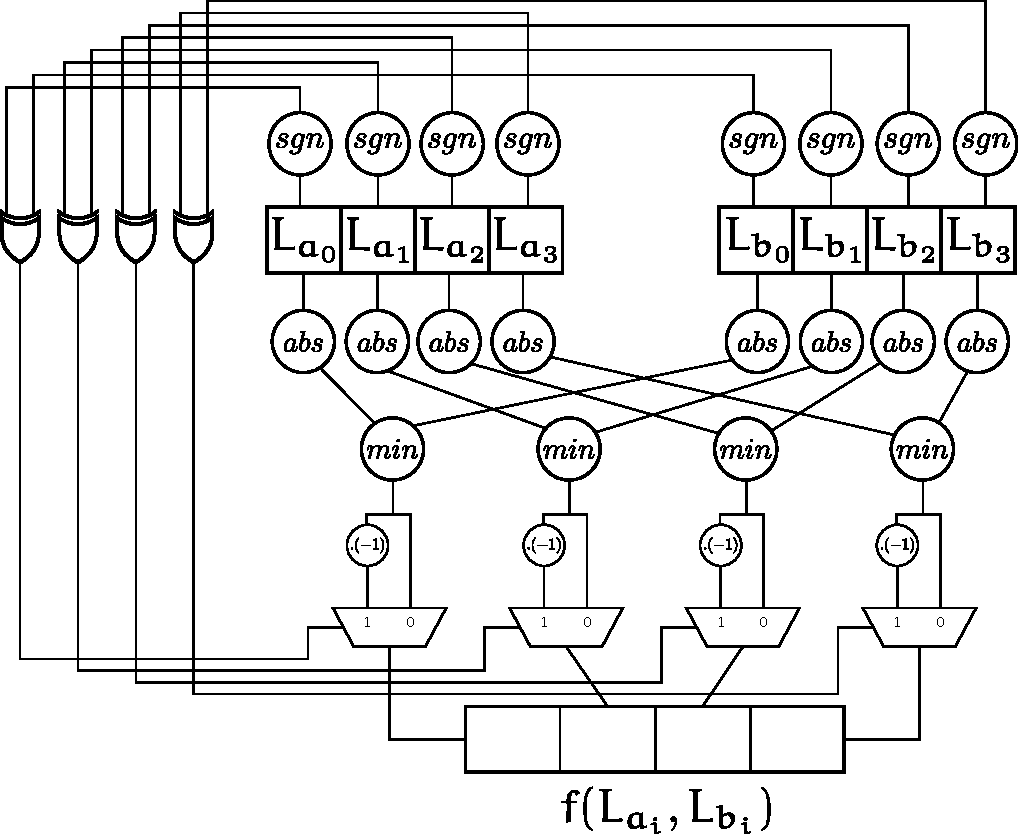
\includegraphics[scale=0.45]{main/ch3_fig/f_tie}
  \label{fig:f_tie}
  }
  \subfloat[Fonction $g$]{
  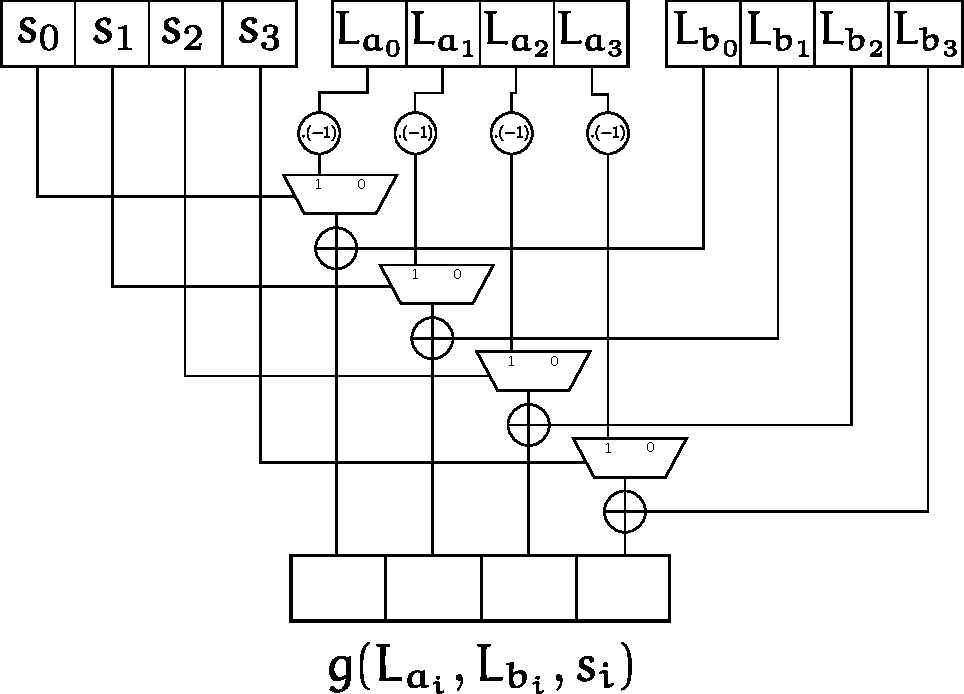
\includegraphics[scale=0.45]{main/ch3_fig/g_tie}
  \label{fig:g_tie}
  }
  \caption{Unités matérielles des fonctions $f$ et $g$}
\end{figure}
\subsubsection{Implémentation matérielle}
La conception des instructions spécialisées est basée sur les unités matérielles décrites dans la littérature des implémentations matérielles de l'algorithme SC décrites en Section \ref{subsec:sota_sc}. Ces instructions spécialisées sont donc décrites à l'aide du langage TIE de Tensilica.
L'implémentation de la fonction $f$ est représentée dans la Figure~\ref{f_tie}. Les deux entrées sont les LLRs notés $L_a$ et $L_b$ et la sortie est notée $f(L_a,L_b)$. Souvent, pour réduire le chemin critique, les LLRs sont représentés en \og signe-amplitude \fg : un bit est utilisé pour le signe, et le reste pour la valeur absolue, toujours positive. Dans notre implémentation, les valeurs négatives sont représentées en complément à deux, car il s'agit du mode de représentation utilisé dans les processeurs XTensa.
La fonction $g$ est représentée dans la Figure~\ref{g_tie}. Elle consiste en une addition simple avec une inversion de signe selon la valeur de la somme partielle $s_a$.
La fonction $h$ n'est pas représentée, il s'agit simplement d'un ou-exclusif entre les sommes partielles d'entrées. Les fonctions \texttt{R0} et \texttt{R1} sont également très simples est leur représentation graphique n'est pas utile, puisqu'il s'agit d'une mise à zéro dans le premier cas, et d'un seuillage dans le deuxième, c'est à dire une simple copie du bit de poids fort.

Comme présenté dans la Section~\ref{subsec:pruning}, le traitement d'un \noeud de répétition consiste en l'addition de tous les LLRs d'entrée pour former la variable notée \og \texttt{accum} \fg dans la Figure~\ref{fig:rep_tie}. Puis de la détection du signe de cette variable, qui détermine le vecteur $s$ en sortie. Un arbre binaire est parcouru afin de réaliser l'addition nécessaire. Pour éviter tout débordement, la taille du registre de stockage de la variable \texttt{accum} est de 32 bits.

L'unité matérielle de traitement des \noeuds \texttt{SPC} est représentée dans la Figure~\ref{fig:spc_tie}

\subsubsection{Unités matérielles \textit{in-register}}

Dans les implémentations logicielles classiques, la séquence d'opérations nécessaire à l'exécution des fonctions élémentaires polaires est la suivante : i) chargement depuis la mémoire cache vers les registres des variables d'entrée (LLRs et / ou sommes partielles), ii) calcul du résultat de la fonction élémentaire, en une ou plusieurs étapes, dont la sortie est stockée dans un registre, iii) sauvegarde de cette variable de sortie dans la mémoire cache du processeur.

\`A l'inverse, dans les implémentations matérielles, il n'y a pas dans registre, dans le sens où le chemin de données part de la sortie de la mémoire, passe par les fonctions combinatoires réalisant les fonctions élémentaires, et finit à l'entrée de la mémoire. Ce chemin de données est parcouru en un coup d'horloge. La méthode présentée dans cette section, nommée \textit{in-register}, est conçue dans le but de reproduire le fonctionnement des implémentations matérielles de code polaire dans notre processeur.

\begin{figure}[t]
\centering
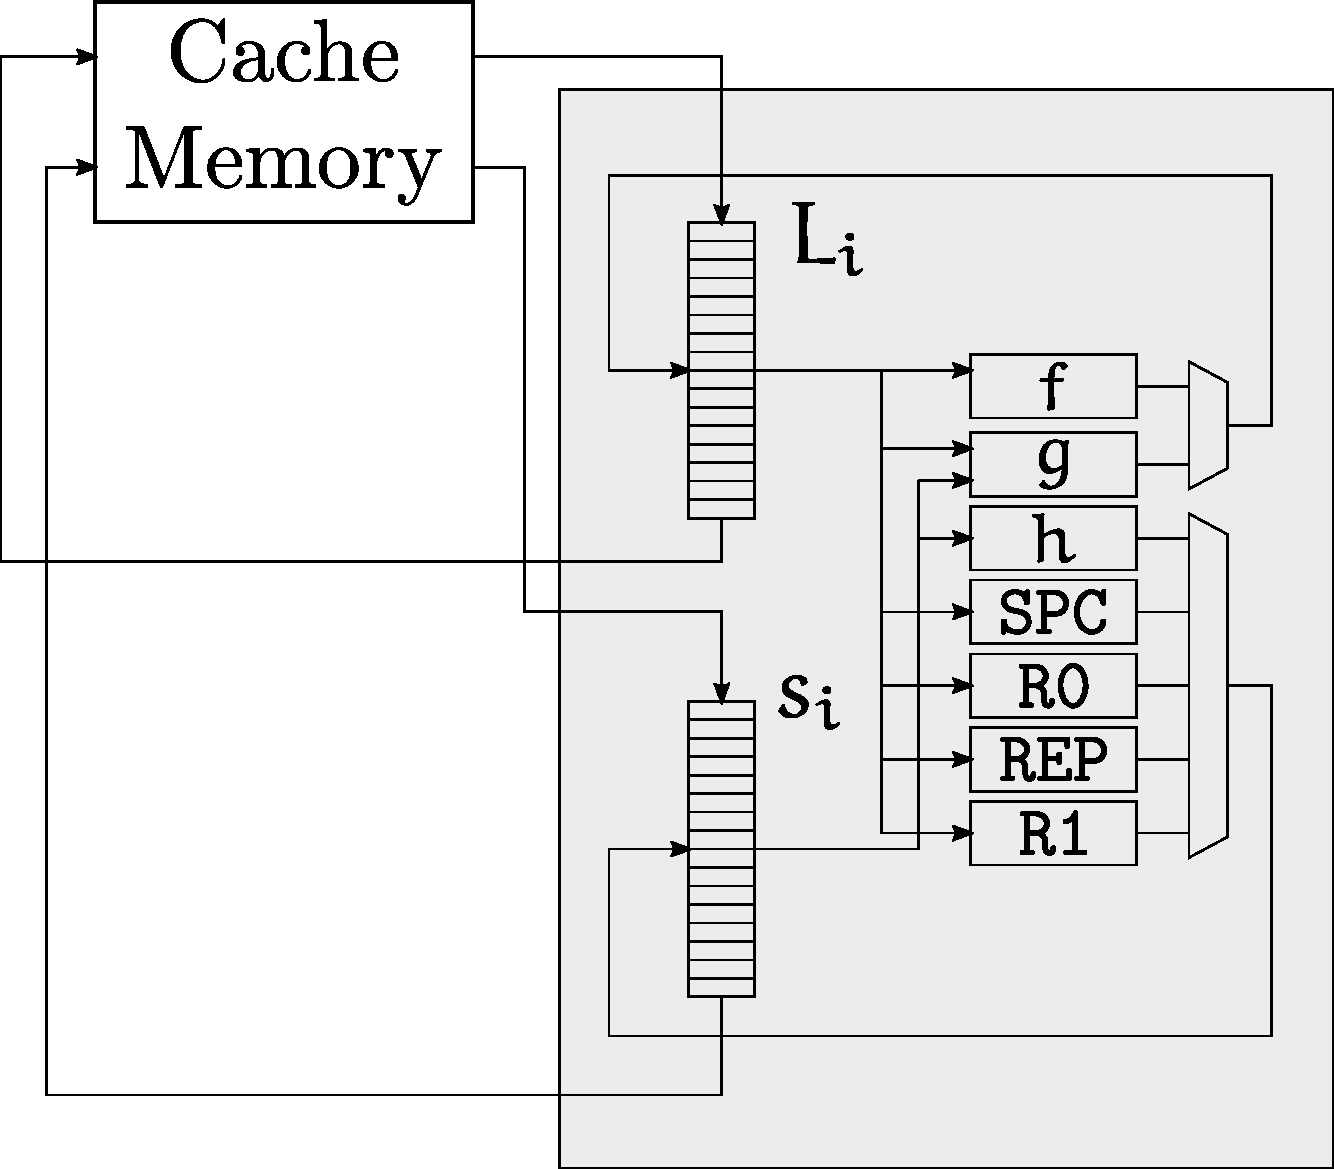
\includegraphics[width=0.7\textwidth]{main/ch3_fig/in_register}
\caption{Instructions \textit{in-register}}
\label{fig:in-register}
\end{figure}

La méthode \textit{in-register} est appliquée sur les sous-arbres de décodage dont le \noeud racine a une taille inférieure à 512 bits.
Lorsque le programme a généré les LLRs de la racine de ce sous-arbre, ceux-ci sont stockés dans un registre dédié.
Ce registre est noté $\mathbold{L}$ dans la Figure~\ref{fig:in-register} qui illustre la méthode.
Le décodage du sous-arbre se fait ensuite intégralement dans les registres, sans passer par la mémoire cache.
Cette méthode reproduit donc comme voulu le fonctionnement des implémentations matérielles de l'algorithme SC : l'exécution d'une fonction élémentaires quelconque, comprenant la lecture et l'écriture de la donnée, peut se faire en un coup d'horloge seulement.

Elle résout également un problème récurrent des implémentations logicielles utilisant du parallélisme : l'alignement des données. En effet, pour pouvoir appliquer une fonction vectorielle des données de deux registres vectoriels, il est nécessaire de les aligner, ce qui nécessite d'effectuer des opérations supplémentaires. Dans l'implémentation \textit{in-register}, l'alignement est prévu en amont et implémenté dans l'unité matérielle. Aucune instruction supplémentaire n'est nécessaire. 

\subsection{Description logicielle}
Lors du développement, il est apparu qu'il était difficile de réduire le temps passé à réaliser les opérations liées au parcours de l'arbre et aux différents tests. L'utilisation de l'option FLIX3 a permis de réduire ce temps, mais pas suffisamment. La technique de déroulage présentée en Section~\ref{subsec:unroll} permet de réduire ce temps. Dérouler le code signifie sacrifier en flexibilité. En effet, il faut générer une version différente du code pour un ensemble donné de paramètres.

Une alternative est utilisée dans l'implémentation proposée. Tout d'abord, toutes les fonctions élémentaires pour le décodage de code polaires possèdent le même prototype de fonctions dans la description logicielle. Le type de fonction à appliquer ($f$, $g$, $h$, \texttt{R0}, \texttt{R1}, \texttt{SPC}, \texttt{REP}) est passé en paramètre de la fonction, accompagné des adresses auxquelles accéder aux données à lire et écrire. De cette manière, il est possible de créer, un tableau contenant les pointeurs des fonctions à appeler. L'algorithme permettant de déterminer la séquence de fonctions à exécuter prend comme entrée le tableau de bits gelés correspondant au code polaire traité.

\section{Expérimentations et mesures}
\label{sec:tensilica_res}

Les codes polaires considérés ont été construits selon le document spécifiant les techniques de modulation et de codage pour le standard 5G \cite{}. 
La version académique des outils de design de Tensilica ne permettent pas d'effectuer une synthèse logique du processeur ou d'accéder à sa description RTL. Seules des estimations de la fréquence, de la consommation et de l'aire occupée sont données. En sélectionnant la technologie HPM 28nm de TSMC, la puissance consommée estimée pour l'ASIP est de 111 mW, et l'aire occupée est 0.475 mm\textsuperscript{2}. La fréquence estimée est 835 MHz. Cependant, les instructions spécialisées ne sont pas prises en compte pour l'estimation de la fréquence. En conséquence, un scénario plus pessimiste où la fréquence de fonctionnement est 400 MHz est également présentée. Avec cette fréquence réduite, la consommation estimée devient XXX mW et l'aire occupée XXX mm\textsuperscript{2}.
\subsection{Comparaison avec un processeur ARM}
Le logiciel AFF3CT développé par l'équipe CSN du laboratoire IMS de Bordeaux est utilisé pour exécuter une implémentation optimisée de l'algorithme SC sur un processeur ARM Cortex A57. La méthode de parallélisation \textit{intra-trame} est utilisée, et les LLRs sont représentés sur 8 bits avec virgule fixe. La taille des données gérées par les instructions NEON est de 128 bits, donc le parallélisme est égal à 16. Les résultats ici reportés ont été fournis par les auteurs de \cite{cassagne_energy_2016}. Dans ces résultats, la consommation de la mémoire RAM n'est pas prise en compte.
La Figure~\ref{fig:cycle_count} montre le nombre moyens de coups d'horloges nécessaire à chaque processeur pour décoder une trame. Le processeur proposé réduit significativement grâce à l'utilisation d'unités matérielles de calcul spécialisées. La courbe tracée représente le rapport entre les nombres de cycle d'horloge de chaque processeur. Ce rapport est d'autant plus grand que $N$ est faible. Ceci est dû au fait que lorsque $N$ est faible, ce sont les instructions \textit{en registre} qui sont le plus utilisées. Or ces instructions sont les plus efficaces.
Cependant, ce nombre réduit de coups d'horloge est contrebalancé par une fréquence réduite comme montré dans le Tableau~\ref{tab:asip}. Néanmoins, même dans le scénario le plus pessimiste, avec une fréquence de 400 MHz, le débit atteint par le processeur proposé est similaire à celui obtenu avec le processeur ARM. Qui plus est, l'énergie dépensée par bit décodé est 10 fois inférieur pour l'ASIP.

\subsection{Comparaison avec un processeur d'architecture x86}
Les débits, latences et l'énergie consommée par bit du décodeur logiciel SC inclus dans le logiciel aff3ct ont également été mesurées sur un processeur Intel i7-4712HQ.
La puissance du \coeur est évaluée avec l'outil \texttt{powergadget} d'Intel. Seule la consommation du \coeur du processeur, excluant la consommation de la mémoire cache de niveau 3 et de la mémoire externe, est reportée. Cette fois-ci, le niveau de parallélisme est de 32 grâce à l'utilisation des instructions AVX2. La fréquence du CPU mesurée durant l'exécution est de 3.3 GHz. Les résultats montrent que le débit et la latence des implémentations de décodeur SC sur les processeurs i7 sont bien meilleurs que ceux obtenus avec le processeur ASIP proposé ou avec le processeur ARM. Cependant, la consommation énergétique est moins bonne. Une implémentation \textit{inter-trame} permettrait d'augmenter cette efficacité énergétique, au prix d'une augmentation de la latence, comme démontré dans \cite{cassagne_energy_2016}.


\begin{table}
  \centering
  \caption{Comparison of the latency, throughput and power consumption}
  \label{tab:asip}
%\scriptsize
  \begin{tabular}{ccccc}
    \toprule

    Target & $N$ & \begin{tabular}{c}Latency\\{[$\mu$s]}\end{tabular} & \begin{tabular}{c}Throughput\\{[Mb/s]}\end{tabular} & \begin{tabular}{c}$E_b$\\{[nJ]}\end{tabular} \\

    \cmidrule(lr){1-1}
    \cmidrule(lr){2-2}
    \cmidrule(lr){3-5}

    \multirow{4}{*}{\bf A57-1.1GHz}
     & $1024$  & $13$  & $38$  & $21$  \\
     & $512$   & $6.7$ & $38$  & $21$  \\
     & $256$   & $3.6$ & $35$  & $22$  \\
     & $128$   & $2.1$ & $30$  & $27$  \\
    \midrule
    \multirow{4}{*}{\bf i7-3.3GHz}
     & $1024$  & $2.3$ & $222$ & $47$  \\
     & $512$   & $1.4$ & $182$ & $57$  \\
     & $256$   & $0.8$ & $155$ & $68$  \\
     & $128$   & $0.5$ & $124$ & $85$  \\
    \midrule
    \multirow{4}{*}{\bf ASIP-835MHz}
     & $1024$  & $7.2$ & $71$  & $1.6$ \\
     & $512$   & $3.9$ & $66$  & $1.7$ \\
     & $256$   & $1.9$ & $65$  & $1.7$ \\
     & $128$   & $1.0$ & $62$  & $1.8$ \\
    \midrule
    \multirow{4}{*}{\bf ASIP-400MHz}
     & $1024$  & $15$ &  $34$  & $1.4$ \\
     & $512$   & $8.2$ & $31$  & $1.6$ \\
     & $256$   & $4.1$ & $31$  & $1.6$ \\
     & $128$   & $2.1$ & $30$  & $1.7$ \\
    \bottomrule
  \end{tabular}
\end{table}

\subsection{Estimation de complexité}
\subsection{Comparaisons}

\section*{Conclusion}

